% 图 74.1 —— 由 `checks/emit_hand.py` 自动拼出（probe 精测 + prims2 图元分解）
%%
% ⚠ 这是**稿子不是成品**：跑 `checks/checkhand.py 74.1` 看指标 + 看叠合图。
%%
%% ⚠ 待核：
%   · 本图 probe 报出阴影族 2 个 —— **本脚本不生成阴影**（要照原书手写）；prims2 的 strokes 里可能含阴影线，核对时留意别画重
%   · 可疑字形 1 项（空心圈 ⊙ 常被认成字母 o）—— 见文件末
%%
\documentclass[12pt]{standalone}
\usepackage{fontspec}
\setsansfont{Arial}
\newfontfamily\mfallback{DejaVu Sans}
\usepackage{tikz}
\begin{document}
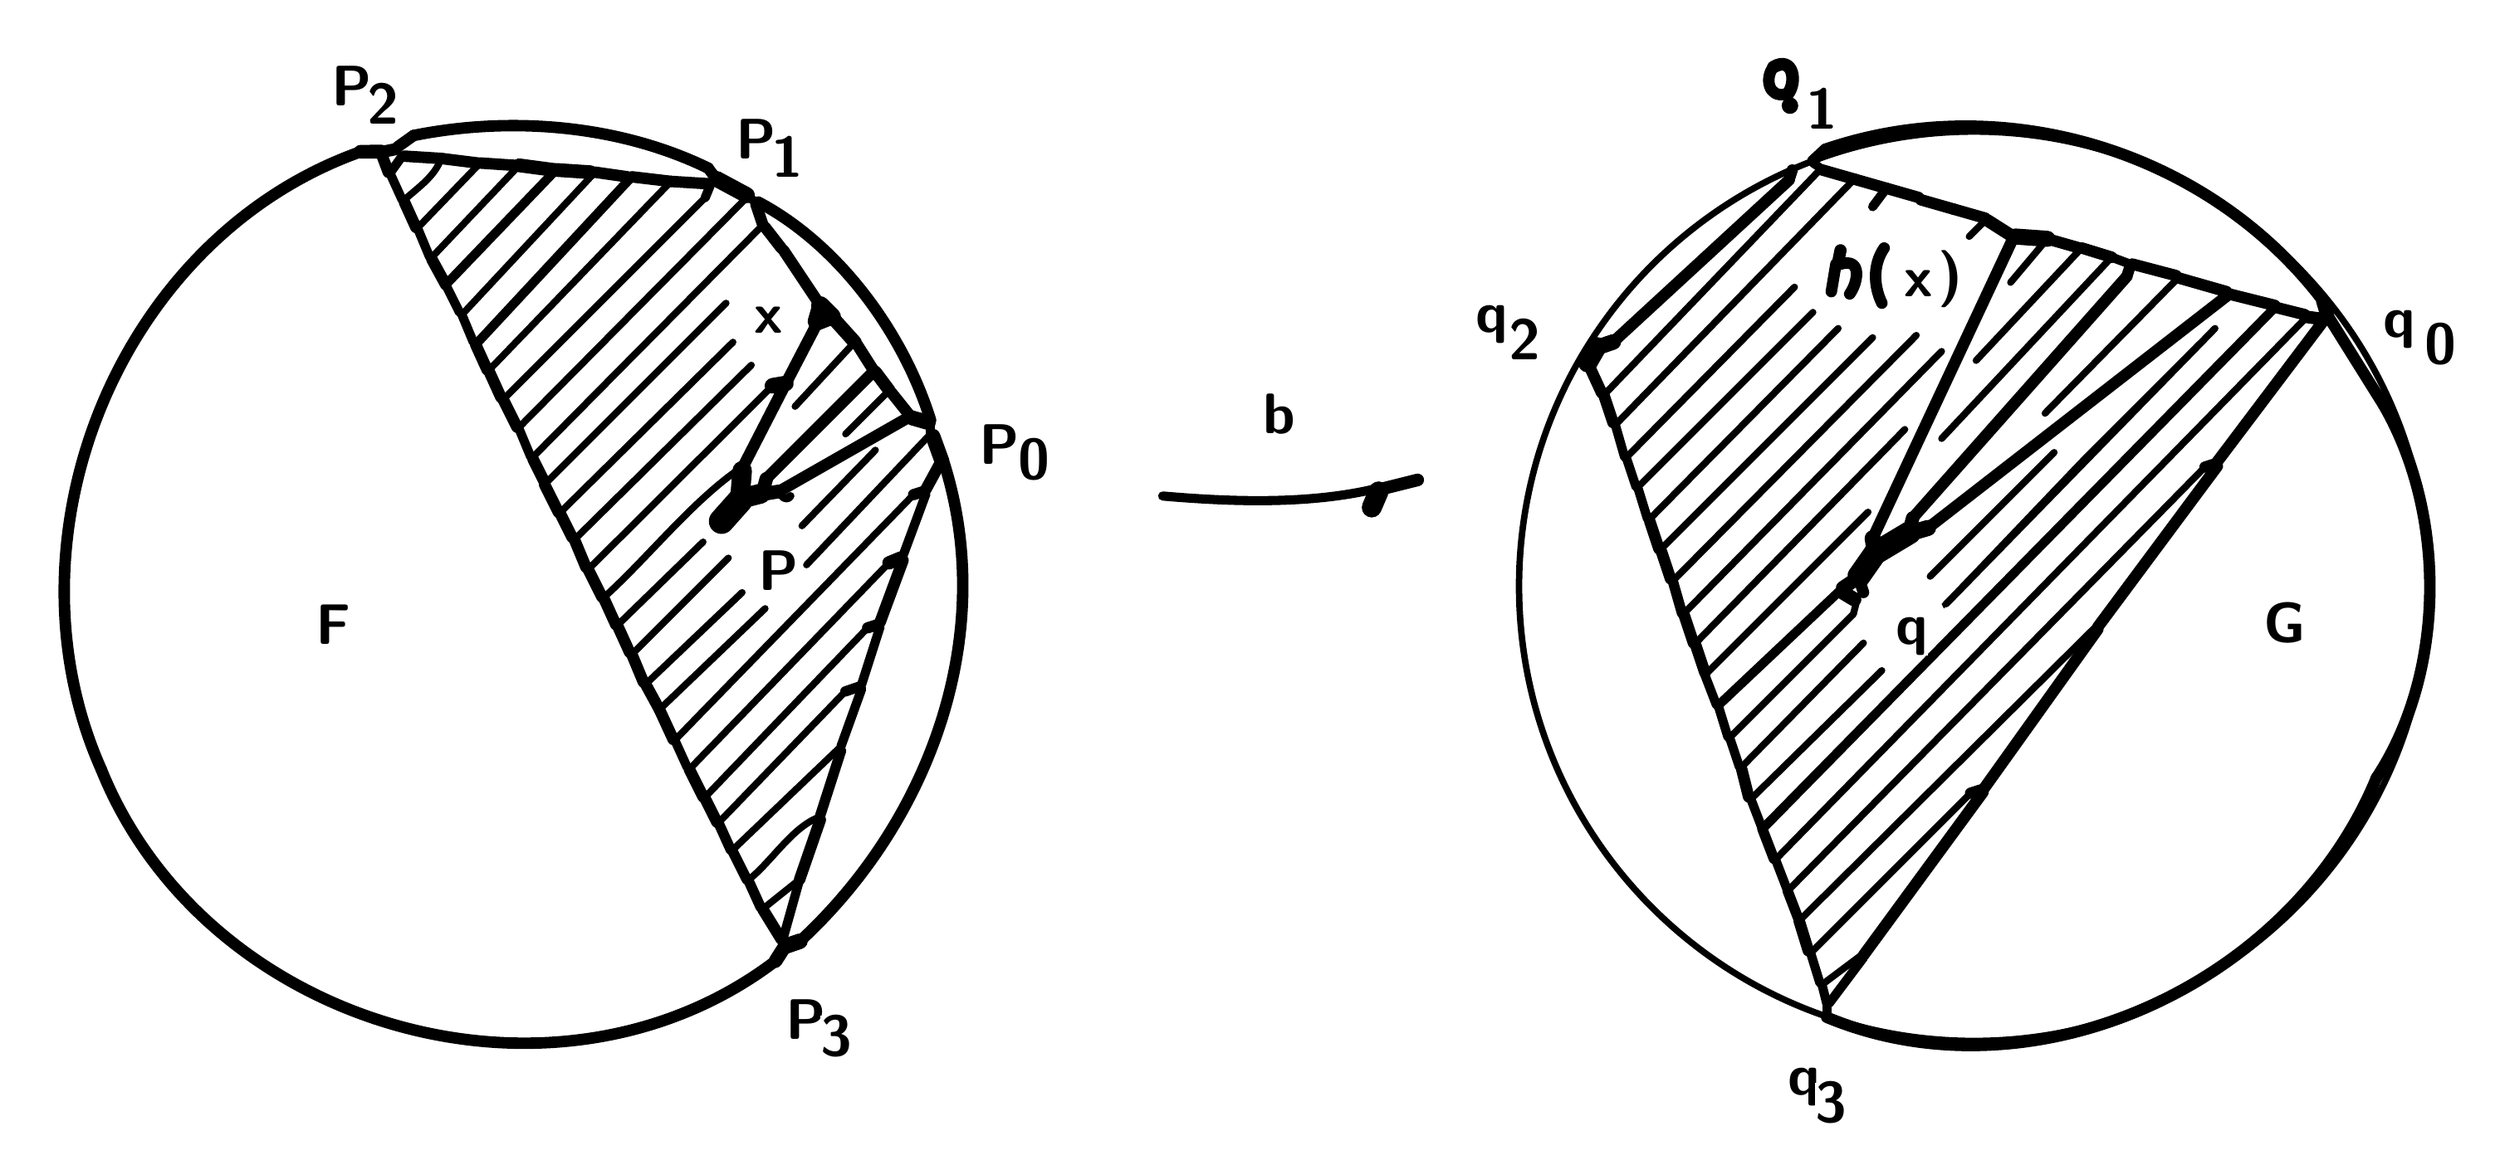
\begin{tikzpicture}[x=1pt, y=-1pt, line width=2.8pt, line cap=round, line join=round]

  %% ════ 填充区（prims2 的 fills）════
  \fill (954.0,133.0) -- (946.0,139.0) -- (897.0,188.0) -- (835.0,253.0) -- (836.0,255.0) -- (947.0,142.0) -- cycle;

  %% ════ 直线段（prims2 的 strokes）════
  \draw[line width=5.0pt] (811.0,72.0) -- (797.0,68.0);
  \draw[line width=5.0pt] (811.0,72.0) -- (825.0,76.0);
  \draw[line width=4.0pt] (811.0,72.0) -- (805.0,80.0);
  \draw[line width=4.0pt] (757.0,351.0) -- (752.0,338.0);
  \draw[line width=4.0pt] (757.0,351.0) -- (979.0,125.0);
  \draw[line width=4.5pt] (757.0,351.0) -- (762.0,364.0);
  \draw[line width=6.0pt] (156.0,56.0) -- (146.9,56.1);
  \draw[line width=6.0pt] (327.5,408.5) -- (331.0,403.0);
  \draw[line width=4.5pt] (722.0,257.0) -- (718.0,243.0);
  \draw[line width=5.0pt] (171.0,89.0) -- (166.0,78.0);
  \draw[line width=3.0pt] (234.0,213.0) -- (309.0,139.0);
  \draw[line width=3.0pt] (748.0,324.0) -- (801.0,270.0);
  \draw[line width=3.0pt] (790.0,133.0) -- (708.0,216.0);
  \draw[line width=8.5pt] (312.0,207.0) -- (313.0,195.0);
  \draw[line width=3.0pt] (895.0,99.0) -- (850.0,147.0);
  \draw[line width=4.0pt] (172.0,90.0) -- (177.0,102.0);
  \draw[line width=5.0pt] (993.0,127.0) -- (981.0,124.0);
  \draw[line width=5.0pt] (296.0,337.0) -- (290.0,325.0);
  \draw[line width=4.9pt] (301.0,67.0) -- (298.2,63.2);
  \draw[line width=5.0pt] (170.0,49.0) -- (163.0,54.0);
  \draw[line width=5.0pt] (234.0,214.0) -- (239.0,224.0);
  \draw[line width=5.0pt] (1027.3,166.3) -- (1004.0,129.0);
  \draw[line width=3.8pt] (319.0,78.0) -- (316.0,76.0);
  \draw[line width=10.0pt] (821.0,222.0) -- (806.0,231.0);
  \draw[line width=3.0pt] (847.0,93.0) -- (853.0,87.0);
  \draw[line width=5.0pt] (692.0,174.0) -- (688.0,162.0);
  \draw[line width=5.0pt] (728.0,271.0) -- (732.0,283.0);
  \draw[line width=5.5pt] (371.0,152.0) -- (377.0,160.0);
  \draw[line width=4.9pt] (770.0,64.0) -- (768.6,68.4);
  \draw[line width=5.0pt] (768.6,68.4) -- (692.1,138.9);
  \draw[line width=6.8pt] (692.1,138.9) -- (686.0,141.0);
  \draw[line width=3.0pt] (830.0,241.0) -- (884.0,187.0);
  \draw[line width=4.0pt] (264.0,68.0) -- (198.0,139.0);
  \draw[line width=5.0pt] (712.0,229.0) -- (708.0,217.0);
  \draw[line width=8.7pt] (587.0,211.0) -- (590.0,204.0);
  \draw[line width=5.0pt] (323.0,89.0) -- (330.0,98.0);
  \draw[line width=5.0pt] (909.0,102.0) -- (896.0,98.0);
  \draw[line width=4.0pt] (909.0,102.0) -- (917.0,105.0);
  \draw[line width=3.0pt] (909.0,102.0) -- (835.0,181.0);
  \draw[line width=6.0pt] (792.0,246.0) -- (798.0,242.0);
  \draw[line width=5.0pt] (713.0,230.0) -- (717.0,242.0);
  \draw[line width=4.5pt] (321.0,385.0) -- (316.0,374.0);
  \draw[line width=5.0pt] (222.0,190.0) -- (227.0,200.0);
  \draw[line width=5.0pt] (233.0,213.0) -- (227.0,201.0);
  \draw[line width=3.0pt] (689.0,161.0) -- (782.0,64.0);
  \draw[line width=4.9pt] (372.0,262.0) -- (367.6,263.4);
  \draw[line width=3.0pt] (367.6,263.4) -- (297.0,337.0);
  \draw[line width=4.0pt] (356.0,315.0) -- (365.0,290.0);
  \draw[line width=5.0pt] (799.0,242.0) -- (801.0,248.0);
  \draw[line width=5.0pt] (783.0,64.0) -- (797.0,68.0);
  \draw[line width=3.0pt] (216.0,176.0) -- (315.0,76.0);
  \draw[line width=5.0pt] (277.0,299.0) -- (271.0,288.0);
  \draw[line width=3.0pt] (277.0,299.0) -- (323.0,255.0);
  \draw[line width=5.0pt] (277.0,299.0) -- (283.0,312.0);
  \draw[line width=5.0pt] (370.0,152.0) -- (323.5,198.5);
  \draw[line width=5.9pt] (323.5,198.5) -- (322.0,204.0);
  \draw[line width=5.0pt] (338.0,373.0) -- (347.0,347.0);
  \draw[line width=3.0pt] (338.0,373.0) -- (323.0,385.0);
  \draw[line width=4.0pt] (338.0,373.0) -- (331.0,398.0);
  \draw[line width=4.0pt] (231.0,65.0) -- (184.0,114.0);
  \draw[line width=5.0pt] (789.0,105.0) -- (787.0,117.0);
  \draw[line width=6.5pt] (394.0,174.0) -- (387.0,172.0);
  \draw[line width=4.0pt] (782.0,418.0) -- (778.0,405.0);
  \draw[line width=6.8pt] (332.0,157.0) -- (326.2,158.0);
  \draw[line width=3.0pt] (326.2,158.0) -- (247.0,237.0);
  \draw[line width=5.0pt] (332.0,157.0) -- (345.0,132.0);
  \draw[line width=5.0pt] (332.0,157.0) -- (313.0,194.0);
  \draw[line width=5.0pt] (840.0,81.0) -- (826.0,77.0);
  \draw[line width=5.0pt] (840.0,81.0) -- (854.0,85.0);
  \draw[line width=5.0pt] (209.0,164.0) -- (215.0,176.0);
  \draw[line width=3.0pt] (198.0,62.0) -- (172.0,89.0);
  \draw[line width=4.5pt] (773.0,391.0) -- (768.0,378.0);
  \draw[line width=3.0pt] (773.0,391.0) -- (902.0,263.0);
  \draw[line width=5.0pt] (773.0,391.0) -- (777.0,404.0);
  \draw[line width=5.0pt] (393.0,203.0) -- (399.0,192.0);
  \draw[line width=3.0pt] (341.0,236.0) -- (394.0,180.0);
  \draw[line width=4.5pt] (315.0,373.0) -- (309.0,361.0);
  \draw[line width=3.8pt] (782.0,63.0) -- (779.0,61.0);
  \draw[line width=4.0pt] (785.0,428.0) -- (785.0,432.0);
  \draw[line width=5.0pt] (203.0,152.0) -- (208.0,163.0);
  \draw[line width=5.0pt] (263.0,67.0) -- (249.0,65.0);
  \draw[line width=5.0pt] (322.0,88.0) -- (319.0,79.0);
  \draw[line width=7.0pt] (881.0,94.0) -- (867.0,93.0);
  \draw[line width=5.0pt] (881.0,94.0) -- (895.0,98.0);
  \draw[line width=3.0pt] (881.0,94.0) -- (865.0,113.0);
  \draw[line width=5.0pt] (331.0,99.0) -- (347.0,123.0);
  \draw[line width=4.0pt] (365.0,288.0) -- (373.0,263.0);
  \draw[line width=5.3pt] (162.0,55.0) -- (157.0,56.0);
  \draw[line width=3.0pt] (336.0,167.0) -- (361.0,140.0);
  \draw[line width=4.0pt] (702.0,202.0) -- (698.0,190.0);
  \draw[line width=5.0pt] (270.0,287.0) -- (265.0,275.0);
  \draw[line width=5.0pt] (938.0,111.0) -- (959.0,117.0);
  \draw[line width=6.5pt] (400.0,191.0) -- (396.0,180.0);
  \draw[line width=6.0pt] (362.0,139.0) -- (353.0,129.0);
  \draw[line width=5.5pt] (1001.0,129.0) -- (994.0,128.0);
  \draw[line width=3.0pt] (296.0,226.0) -- (259.0,262.0);
  \draw[line width=5.0pt] (363.0,140.0) -- (370.0,151.0);
  \draw[line width=4.0pt] (190.0,126.0) -- (184.0,114.0);
  \draw[line width=3.0pt] (880.0,170.0) -- (937.0,112.0);
  \draw[line width=6.8pt] (338.1,399.9) -- (332.0,402.0);
  \draw[line width=5.0pt] (918.0,105.0) -- (937.0,110.0);
  \draw[line width=3.0pt] (291.0,324.0) -- (376.9,235.1);
  \draw[line width=5.8pt] (376.9,235.1) -- (382.0,233.0);
  \draw[line width=5.0pt] (687.0,161.0) -- (681.0,148.0);
  \draw[line width=5.0pt] (751.0,337.0) -- (748.0,325.0);
  \draw[line width=5.0pt] (853.0,334.0) -- (903.0,264.0);
  \draw[line width=8.7pt] (321.0,205.0) -- (313.0,207.0);
  \draw[line width=5.0pt] (723.0,258.0) -- (727.0,270.0);
  \draw[line width=5.0pt] (184.0,114.0) -- (178.0,103.0);
  \draw[line width=11.0pt] (304.0,217.0) -- (312.0,208.0);
  \draw[line width=3.0pt] (743.0,311.0) -- (796.6,257.4);
  \draw[line width=3.0pt] (796.6,257.4) -- (798.0,252.0);
  \draw[line width=5.0pt] (297.0,338.0) -- (302.0,348.0);
  \draw[line width=3.0pt] (178.0,102.0) -- (215.0,63.0);
  \draw[line width=4.0pt] (693.0,175.0) -- (697.0,189.0);
  \draw[line width=5.0pt] (866.0,94.0) -- (805.0,224.4);
  \draw[line width=7.0pt] (805.0,224.4) -- (806.0,231.0);
  \draw[line width=8.0pt] (352.0,128.0) -- (347.0,123.0);
  \draw[line width=5.0pt] (330.0,399.0) -- (322.0,386.0);
  \draw[line width=5.0pt] (329.0,204.0) -- (385.0,172.0);
  \draw[line width=6.0pt] (329.0,204.0) -- (323.0,205.0);
  \draw[line width=3.0pt] (376.0,161.0) -- (358.0,179.0);
  \draw[line width=5.3pt] (790.0,104.0) -- (791.0,99.0);
  \draw[line width=4.0pt] (783.0,419.0) -- (785.0,427.0);
  \draw[line width=3.0pt] (805.0,137.0) -- (713.0,229.0);
  \draw[line width=4.9pt] (852.0,334.0) -- (847.6,335.4);
  \draw[line width=3.0pt] (847.6,335.4) -- (779.0,404.0);
  \draw[line width=5.0pt] (245.0,237.0) -- (240.0,225.0);
  \draw[line width=6.0pt] (1003.0,128.0) -- (1000.9,120.9);
  \draw[line width=5.0pt] (784.4,55.0) -- (779.0,60.0);
  \draw[line width=4.0pt] (707.0,216.0) -- (703.0,203.0);
  \draw[line width=3.0pt] (284.0,312.0) -- (387.6,205.4);
  \draw[line width=4.9pt] (387.6,205.4) -- (392.0,204.0);
  \draw[line width=5.0pt] (246.0,238.0) -- (252.0,250.0);
  \draw[line width=3.0pt] (698.0,189.0) -- (771.0,115.0);
  \draw[line width=3.0pt] (228.0,200.0) -- (306.0,122.0);
  \draw[line width=3.0pt] (266.0,274.0) -- (307.0,233.0);
  \draw[line width=3.0pt] (719.0,242.0) -- (824.0,136.0);
  \draw[line width=4.0pt] (216.0,177.0) -- (221.0,189.0);
  \draw[line width=4.0pt] (160.0,65.0) -- (165.0,58.0);
  \draw[line width=5.0pt] (156.0,57.0) -- (159.0,65.0);
  \draw[line width=4.0pt] (747.0,324.0) -- (743.0,312.0);
  \draw[line width=4.0pt] (395.0,175.0) -- (395.0,179.0);
  \draw[line width=3.0pt] (733.0,283.0) -- (803.0,213.0);
  \draw[line width=3.0pt] (339.0,219.0) -- (371.0,186.0);
  \draw[line width=8.4pt] (685.0,141.0) -- (681.0,148.0);
  \draw[line width=5.0pt] (903.0,263.0) -- (955.0,193.0);
  \draw[line width=6.0pt] (216.0,62.0) -- (231.0,64.0);
  \draw[line width=3.0pt] (309.0,360.0) -- (355.0,316.0);
  \draw[line width=5.5pt] (591.0,203.0) -- (607.0,199.0);
  \draw[line width=3.0pt] (241.0,224.0) -- (317.0,149.0);
  \draw[line width=7.0pt] (347.0,123.0) -- (345.0,130.0);
  \draw[line width=3.0pt] (303.0,348.0) -- (357.9,291.1);
  \draw[line width=4.5pt] (357.9,291.1) -- (364.0,289.0);
  \draw[line width=4.0pt] (738.0,298.0) -- (742.0,311.0);
  \draw[line width=4.0pt] (191.0,127.0) -- (196.0,139.0);
  \draw[line width=10.0pt] (806.0,231.0) -- (799.0,241.0);
  \draw[line width=3.0pt] (797.0,68.0) -- (694.0,174.0);
  \draw[line width=5.0pt] (980.0,123.0) -- (960.0,118.0);
  \draw[line width=5.7pt] (346.0,131.0) -- (351.0,129.0);
  \draw[line width=4.9pt] (954.0,192.0) -- (949.6,193.4);
  \draw[line width=3.0pt] (949.6,193.4) -- (768.0,378.0);
  \draw[line width=4.0pt] (738.0,297.0) -- (791.0,247.0);
  \draw[line width=3.0pt] (321.0,89.0) -- (222.0,189.0);
  \draw[line width=5.0pt] (258.0,262.0) -- (253.0,251.0);
  \draw[line width=3.0pt] (763.0,364.0) -- (993.0,129.0);
  \draw[line width=5.0pt] (182.0,59.0) -- (166.0,58.0);
  \draw[line width=5.0pt] (182.0,59.0) -- (198.0,61.0);
  \draw[line width=5.0pt] (801.0,406.0) -- (853.0,335.0);
  \draw[line width=5.0pt] (1001.0,130.0) -- (955.0,191.0);
  \draw[line width=6.0pt] (247.0,65.0) -- (232.0,64.0);
  \draw[line width=4.0pt] (737.0,297.0) -- (732.0,284.0);
  \draw[line width=5.0pt] (959.0,119.0) -- (829.1,219.9);
  \draw[line width=7.0pt] (829.1,219.9) -- (822.0,222.0);
  \draw[line width=5.0pt] (298.0,70.0) -- (282.0,69.0);
  \draw[line width=3.0pt] (313.0,248.0) -- (272.0,287.0);
  \draw[line width=3.0pt] (728.0,270.0) -- (819.0,177.0);
  \draw[line width=5.0pt] (199.0,61.0) -- (214.0,62.0);
  \draw[line width=5.0pt] (373.0,261.0) -- (383.0,234.0);
  \draw[line width=4.0pt] (768.0,378.0) -- (763.0,365.0);
  \draw[line width=3.0pt] (809.0,282.0) -- (753.0,337.0);
  \draw[line width=5.0pt] (265.0,67.0) -- (282.0,69.0);
  \draw[line width=4.0pt] (289.0,324.0) -- (284.0,313.0);
  \draw[line width=3.0pt] (210.0,163.0) -- (296.9,76.1);
  \draw[line width=4.0pt] (296.9,76.1) -- (299.0,71.0);
  \draw[line width=4.0pt] (786.0,427.0) -- (801.0,407.0);
  \draw[line width=5.9pt] (821.0,221.0) -- (822.4,215.6);
  \draw[line width=5.0pt] (822.4,215.6) -- (915.6,110.4);
  \draw[line width=4.9pt] (915.6,110.4) -- (917.0,106.0);
  \draw[line width=4.0pt] (160.0,66.0) -- (165.0,77.0);
  \draw[line width=3.0pt] (192.0,126.0) -- (248.0,66.0);
  \draw[line width=6.2pt] (792.0,248.0) -- (797.0,251.0);
  \draw[line width=3.0pt] (203.0,151.0) -- (282.0,69.0);
  \draw[line width=4.5pt] (347.0,345.0) -- (356.0,317.0);
  \draw[line width=3.0pt] (703.0,202.0) -- (779.0,126.0);
  \draw[line width=3.0pt] (954.0,133.0) -- (837.0,253.0);
  \draw[line width=5.0pt] (378.0,161.0) -- (386.0,171.0);
  \draw[line width=5.0pt] (264.0,274.0) -- (259.0,263.0);
  \draw[line width=5.0pt] (202.0,151.0) -- (197.0,140.0);
  \draw[line width=4.5pt] (308.0,360.0) -- (303.0,349.0);
  \draw[line width=5.5pt] (855.0,86.0) -- (866.0,93.0);
  \draw[line width=7.0pt] (315.0,75.0) -- (302.0,68.0);
  \draw[line width=4.0pt] (383.0,232.0) -- (393.0,205.0);
  \draw[line width=3.0pt] (723.0,257.0) -- (835.0,143.0);
  \draw[line width=3.0pt] (784.0,418.0) -- (800.0,406.0);

  %% ════ 曲线（prims2 的 curves —— 三段式，坐标同为 (y,x)）════
  \draw[line width=5.0pt] (146.9,56.1) .. controls (41.5,93.6) and (-10.7,224.2) .. (34.0,324.9);
  \draw[line width=5.0pt] (34.0,324.9) .. controls (79.3,437.5) and (231.6,481.5) .. (327.5,408.5);
  \draw[line width=5.0pt] (298.2,63.2) .. controls (259.8,44.5) and (212.9,40.4) .. (170.0,49.0);
  \draw[line width=5.0pt] (785.0,433.0) .. controls (874.8,470.4) and (987.4,418.6) .. (1024.2,328.8);
  \draw[line width=5.0pt] (1024.2,328.8) .. controls (1054.5,283.0) and (1054.9,213.9) .. (1027.3,166.3);
  \draw[line width=4.0pt] (588.0,203.0) .. controls (559.3,209.7) and (526.0,208.6) .. (496.0,206.0);
  \draw[line width=3.0pt] (312.0,194.0) .. controls (290.7,208.8) and (272.7,232.1) .. (253.0,250.0);
  \draw[line width=5.0pt] (401.0,192.0) .. controls (424.2,266.4) and (395.0,347.4) .. (338.1,399.9);
  \draw[line width=3.5pt] (329.0,204.0) .. controls (329.8,205.9) and (332.0,208.6) .. (334.0,206.0);
  \draw[line width=5.0pt] (1000.9,120.9) .. controls (950.9,55.3) and (861.3,28.6) .. (784.4,55.0);
  \draw[line width=5.0pt] (795.0,118.0) .. controls (798.5,113.3) and (800.7,102.1) .. (791.0,105.0);
  \draw[line width=5.5pt] (768.0,31.0) .. controls (772.2,25.7) and (770.4,14.2) .. (761.8,19.2);
  \draw[line width=5.0pt] (761.8,19.2) .. controls (758.0,23.8) and (759.5,32.7) .. (767.0,31.0);
  \draw[line width=3.0pt] (182.0,59.0) .. controls (179.3,66.8) and (171.8,71.8) .. (166.0,77.0);
  \draw[line width=3.0pt] (346.0,346.0) .. controls (334.3,350.9) and (326.3,364.6) .. (316.0,373.0);
  \draw[line width=5.0pt] (395.0,173.0) .. controls (383.3,135.4) and (355.5,96.8) .. (320.0,78.0);
  \draw[line width=5.0pt] (809.0,122.0) .. controls (805.4,114.6) and (805.0,105.2) .. (810.0,98.0);

  %% ════ 圆 / 椭圆（probe 精测）════
  \draw (849.1,245.3) circle (198.0);

  %% ════ 实心点 ════
  \fill (769.0,36.0) circle (3.6);

  %% ════ 标签（probe 直接给的 \node 行）════
  %% ⚠ 全部补了 fill=white：文字在最上层，否则与曲线交叉干扰
     \node[anchor=center,inner sep=0pt,fill=white,font=\fontsize{29.8}{37.3}\selectfont] at (143.0,27.5) {\textsf{\textbf{\textit{P}}}};   % box(132,15,18,23)
     \node[anchor=center,inner sep=0pt,fill=white,font=\fontsize{25.4}{31.8}\selectfont] at (156.6,35.4) {\textsf{\textbf{2}}};   % box(150,26,12,18)
     \node[anchor=center,inner sep=0pt,fill=white,font=\fontsize{23.7}{29.7}\selectfont] at (782.8,37.4) {\textsf{\textbf{1}}};   % box(776,29,8,16)
     \node[anchor=center,inner sep=0pt,fill=white,font=\fontsize{29.8}{37.3}\selectfont] at (319.0,50.5) {\textsf{\textbf{\textit{P}}}};   % box(308,38,18,23)
     \node[anchor=center,inner sep=0pt,fill=white,font=\fontsize{23.7}{29.7}\selectfont] at (332.8,58.4) {\textsf{\textbf{1}}};   % box(326,50,8,16)
     \node[anchor=center,inner sep=0pt,fill=white,font=\fontsize{28.7}{35.9}\selectfont] at (838.9,111.5) {\textsf{\textbf{)}}};   % box(834,97,7,28)
     \node[anchor=center,inner sep=0pt,fill=white,font=\fontsize{29.2}{36.5}\selectfont] at (825.0,113.4) {\textsf{\textbf{\textit{x}}}};   % box(816,103,16,17)
     \node[anchor=center,inner sep=0pt,fill=white,font=\fontsize{32.0}{40.0}\selectfont] at (639.1,131.4) {\textsf{\textbf{\textit{q}}}};   % box(629,118,18,23)
     \node[anchor=center,inner sep=0pt,fill=white,font=\fontsize{30.1}{37.6}\selectfont] at (324.5,129.5) {\textsf{\textbf{\textit{x}}}};   % box(315,119,17,17)
     \node[anchor=center,inner sep=0pt,fill=white,font=\fontsize{35.4}{44.3}\selectfont] at (1034.2,133.6) {\textsf{\textbf{\textit{q}}}};   % box(1022,120,22,23)
     \node[anchor=center,inner sep=0pt,fill=white,font=\fontsize{24.7}{30.9}\selectfont] at (653.6,137.9) {\textsf{\textbf{2}}};   % box(647,129,12,17)
     \node[anchor=center,inner sep=0pt,fill=white,font=\fontsize{24.9}{31.1}\selectfont] at (1052.1,139.7) {\textsf{\textbf{0}}};   % box(1044,131,12,17)
     \node[anchor=center,inner sep=0pt,fill=white,font=\fontsize{30.0}{37.5}\selectfont] at (546.8,170.2) {\textsf{\textbf{\textit{b}}}};   % box(537,158,17,22)
     \node[anchor=center,inner sep=0pt,fill=white,font=\fontsize{29.8}{37.3}\selectfont] at (425.0,183.5) {\textsf{\textbf{\textit{P}}}};   % box(414,171,18,23)
     \node[anchor=center,inner sep=0pt,fill=white,font=\fontsize{25.6}{32.0}\selectfont] at (440.1,190.2) {\textsf{\textbf{0}}};   % box(432,181,12,18)
     \node[anchor=center,inner sep=0pt,fill=white,font=\fontsize{29.8}{37.3}\selectfont] at (329.0,238.5) {\textsf{\textbf{\textit{P}}}};   % box(318,226,18,23)
     \node[anchor=center,inner sep=0pt,fill=white,font=\fontsize{30.7}{38.3}\selectfont] at (984.2,261.3) {\textsf{\textbf{\textit{G}}}};   % box(974,249,21,23)
     \node[anchor=center,inner sep=0pt,fill=white,font=\fontsize{30.7}{38.4}\selectfont] at (135.0,262.0) {\textsf{\textbf{\textit{F}}}};   % box(125,250,20,22)
     \node[anchor=center,inner sep=0pt,fill=white,font=\fontsize{32.0}{40.0}\selectfont] at (822.1,267.4) {\textsf{\textbf{\textit{q}}}};   % box(812,254,18,23)
     \node[anchor=center,inner sep=0pt,fill=white,font=\fontsize{29.2}{36.4}\selectfont] at (340.9,434.0) {\textsf{\textbf{\textit{P}}}};   % box(330,422,18,22)
     \node[anchor=center,inner sep=0pt,fill=white,font=\fontsize{23.0}{28.7}\selectfont] at (353.9,441.1) {\textsf{\textbf{3}}};   % box(348,432,11,17)
     \node[anchor=center,inner sep=0pt,fill=white,font=\fontsize{32.0}{40.0}\selectfont] at (775.1,463.4) {\textsf{\textbf{\textit{q}}}};   % box(765,450,18,23)
     \node[anchor=center,inner sep=0pt,fill=white,font=\fontsize{23.0}{28.7}\selectfont] at (786.9,470.1) {\textsf{\textbf{3}}};   % box(781,461,11,17)

  % 钉死画布：否则超出的图元/控制点会把页面撑大，1:1 回比就失准
  \pgfresetboundingbox
  \path[use as bounding box] (0,0) rectangle (1068,487);
\end{tikzpicture}
\end{document}

% ⚠ 待核清单（probe 拿不准，人眼过一遍）：
%   · 未识别/跳过：⑤ 跳过/未识别的字形
